\documentclass[12pt]{article}
\usepackage[utf8]{inputenc}
\usepackage[T5]{fontenc}
\usepackage{graphicx,a4wide,framed}

\newcommand{\source}[1]{\begin{flushright}\emph{[#1]}\end{flushright}}

\newcommand{\MakeScribeTop}[1]{
\noindent
\begin{framed}
\noindent
 Algorithmique Avancée 2019
 \hfill
 École Centrale-Supélec
 \\[1em]
 \centerline{ \Large
#1
 }
 \\[1em]
\centerline{  \it Christoph Dürr, Nguyễn Kim Thắng}
\end{framed}
}



\begin{document}
    \MakeScribeTop{PC2 : Programmation dynamique 1}

    \section{Arbre binaire de recherche optimal}

    On veut stocker $n$ éléments comparables dans un arbre binaire de recherche.
    Pour simplifier on suppose que les éléments sont les entiers de $1$ à $n$.
    On pourrait pour cela prendre un arbre binaire équilibré, ce qui garantirait des temps d'accès dans le pire des cas de $O(\log n)$.  Mais on s'intéresse à optimiser le temps d'accès moyen, pour des fréquences d'accès $f[1\ldots n]$ données pour chaque élément.
    Concrètement si $p[i]$ est la profondeur de l'élément $i$ dans l'arbre produit alors on veut minimiser la somme $\sum_{i=1}^n f[i]\cdot p[i]$.
    Pour fixer les choses on dira que la racine a la profondeur $1$, les descendants directs de la racine ont la profondeur $2$ et ainsi de suite.

    Trouvez un algorithme pour ce problème de complexité $O(n^3)$.

\source{Algorithms, Jeff Erickson, section 5.7}

\section{Distance d'édition}

Étant donnée deux mots $x=x_1 \ldots x_n,y=y_1\ldots y_m$ sur un même alphabet, la distance d'édition de Levenshtein est égal au nombre minimum d'insertions, suppressions ou remplacements de lettres que $x$ doit subir pour être transformé en $y$.  Donnez un algorithme en $O(n m)$ pour ce problème.

\section{Corriger un mot bien parenthésé}

Un mot $w$ sur l'alphabet $\Sigma=\{'(',')'\}$  est bien parenthésé si chaque parenthèse ouvrante peut être associé de manière bijective à une parenthésé fermé et que les associations soient sans croisement.  Formellement, $w$ est bien parenthésé s'il est produit par la grammaire $S\rightarrow (S)S | \epsilon $.  Étant donnée un mot $w$ sur $\Sigma$, déterminez en temps $O(n^3)$ le nombre minimum de parenthèses à supprimer pour rendre $w$ bien parenthésé. Qu'en est-il si on autorise également à insérer des parenthèses~?


\section{Parenthéser une expression booléenne}

On vous donne une expression booléenne composée de $n$ constantes $T$ et $F$ (pour vrai et faux), alternant avec $n-1$ opérateurs $\wedge,\vee,\oplus$ (et, ou, ou exclusif).  Comptez le nombre de manières de placer des parenthèses pour que l'ordre d'évaluation soit non ambigu et que l'expression s'évalue à Vrai.  Exemple: l'expression  $T \vee T \wedge F \oplus T$ peut être rendu vraie de 4 manière différentes, à savoir
$((T\vee T)\wedge (F\oplus  T)), (T\vee (T\wedge (F\oplus  T))), (((T\vee T)\wedge F)\oplus  T)$
et $(T\vee ((T\wedge F)\oplus  T))$.

\section{Partage équitable}

Deux voleurs viennent de dérober $n$ objets de valeurs $1\leq w_1,\ldots,w_n \leq M$ respectivement.  Il veulent départager le butin équitablement, c'est à dire trouver un ensemble $S\subseteq \{1,\ldots,n\}$ avec $\sum_{i\in S} w_i$ aussi proche que possible de $\sum_{i\notin S} w_i$.
Donnez un algorithme de complexité polynomiale en $n$ et en $M$.

\section{Rendu de monnaie}


On souhaite obtenir un
montant $R$ avec des billets de banque qui valent respectivement
$x_0,\ldots,x_{n-1}$ Euros. Le problème consiste donc à déterminer s'il existe une combinaison linéaire
positive de $x_0,\ldots,x_{n-1}$ qui vaut $R$. Vous rigolez, mais en Birmanie (aujourd'hui Myanmar), il y
avait des billets de 15, 25, 35, 45, 75 et de 90 kyats.
Pour ce problème, une valeur $x_i$ peut
contribuer plusieurs fois au montant demandé.

\begin{enumerate}
    \item Montrez que l'algorithme glouton, qui sélectionne à chaque fois le plus grand billet ne dépassant pas la somme restante, ne donne pas la bonne solution en général.
\item
Montrez que le même algorithme glouton est optimal pour des billets de valeur $\bigcup_{i=0}^k \{10^i, 2\cdot 10^i, 5\cdot 10^i\}$ pour une constante $k$.
\item
Donnez un programme dynamique pour ce problème de complexité $O(nR)$.
\item
Modifiez le programme pour qu'il donne une solution avec un nombre minimum de billets.
\end{enumerate}
% \begin{figure}[h]
% \centerline{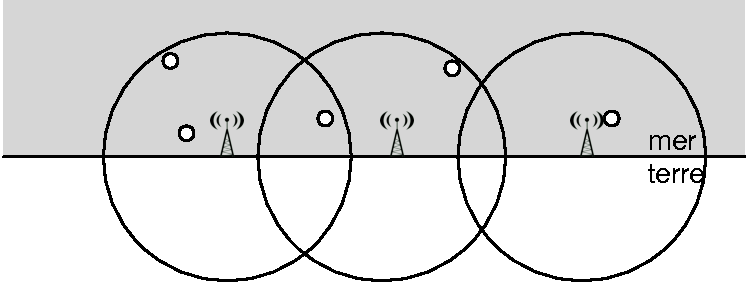
\includegraphics[width=8cm]{radar-disc}}
% \caption{Exemple (non-optimal) de placement d'antennes}
% \end{figure}


\end{document}
